\documentclass[10pt]{article}
 \usepackage[margin=0.5in]{geometry} 
\usepackage{amsmath,amsthm,amssymb, graphicx, multicol, array}
  
\newenvironment{problem}[2][Problem]{\begin{trivlist}
\item[\hskip \labelsep {\bfseries #1}\hskip \labelsep {\bfseries #2.}]}{\end{trivlist}}

\begin{document}
%---------------
%---------------
 \title{Discussion - Light Interference}
\date{}
\maketitle

\begin{problem}{1}
Laser light of 600nm wavelength strikes a double slit and interference is viewed on a screen.
\item (a) If the distance from either slit to the center of the screen is exactly 5m, how many wavelengths fit in between slit and screen?
\item (b) What kind of interference will it be at the center of the screen, and why?
\item (c) One of the slits is completely blocked. What happens to the intensity at the center of the screen?
\item (d) The slit is reopened, but then is covered by a special clear plastic “sandwich”, a $11.800\mu m$-thick middle section of refractive index 2.25 with a 100nm coating of lower refractive index on each side. The coating completely prevents reflection. What is its refractive index?
\item (e) How many wavelengths fit in the sandwich and how many fit in the same
thickness of air? What phase difference results?
\item (f) When covering one slit, the sandwich not only reflects no light, but it absorbs negligible light--all the light striking it passes through--yet the intensity at the center of the screen diminishes significantly. By what fraction?
\end{problem}

\begin{figure}[htp]
    \centering
    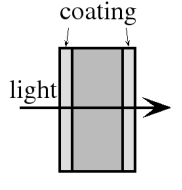
\includegraphics[width=1in]{sandwich.png}
    \caption{Clear Plastic Sandwich}
    \label{fig:Graph of Wave}
\end{figure}






%-------------
%-------------
\end{document}
